\begin{pages}
    \begin{Rightside}
    \selectlanguage{greek}
        \beginnumbering
		\pstart[
				\chapter{Ἰωάννης ἐν τῇ Πάτμῳ}
				\markboth{John on the Isle of Patmos}
				]
		Ἀποκάλυψις Ἰησοῦ Χριστοῦ, ἣν ἔδωκεν αὐτῷ ὁ Θεός, δεῖξαι τοῖς δούλοις αὐτοῦ ἃ δεῖ γενέσθαι ἐν τάχει, καὶ ἐσήμανεν ἀποστείλας διὰ τοῦ ἀγγέλου αὐτοῦ, τῷ δούλῳ αὐτοῦ Ἰωάνῃ, ὃς ἐμαρτύρησεν τὸν λόγον τοῦ Θεοῦ καὶ τὴν μαρτυρίαν Ἰησοῦ Χριστοῦ, ὅσα εἶδεν. Μακάριος ὁ ἀναγινώσκων καὶ οἱ ἀκούοντες τοὺς λόγους τῆς προφητείας καὶ τηροῦντες τὰ ἐν αὐτῇ γεγραμμένα· ὁ γὰρ καιρὸς ἐγγύς.
		\pend
		\pstart
			Ἰωάννης ταῖς ἑπτὰ ἐκκλησίαις ταῖς ἐν τῇ Ἀσίᾳ· χάρις ὑμῖν καὶ εἰρήνη ἀπὸ ὁ ὢν καὶ ὁ ἦν καὶ ὁ ἐρχόμενος, καὶ ἀπὸ τῶν ἑπτὰ Πνευμάτων ἃ ἐνώπιον τοῦ θρόνου αὐτοῦ, καὶ ἀπὸ Ἰησοῦ Χριστοῦ, ὁ μάρτυς ὁ πιστός, ὁ πρωτότοκος τῶν νεκρῶν καὶ ὁ ἄρχων τῶν βασιλέων τῆς γῆς.
		\pend
		\pstart
			Τῷ ἀγαπῶντι ἡμᾶς καὶ λύσαντι ἡμᾶς ἐκ τῶν ἁμαρτιῶν ἡμῶν ἐν τῷ αἵματι αὐτοῦ, καὶ ἐποίησεν ἡμᾶς βασιλείαν, ἱερεῖς τῷ Θεῷ καὶ Πατρὶ αὐτοῦ, αὐτῷ ἡ δόξα καὶ τὸ κράτος εἰς τοὺς αἰῶνας τῶν αἰώνων· ἀμήν.
		\pend
		\pstart	
			Ἰδοὺ ἔρχεται μετὰ τῶν νεφελῶν, καὶ ὄψεται αὐτὸν πᾶς ὀφθαλμὸς καὶ οἵτινες αὐτὸν ἐξεκέντησαν, καὶ κόψονται ἐπ’ αὐτὸν πᾶσαι αἱ φυλαὶ τῆς γῆς. ναί, ἀμήν.
		\pend
		\pstart
			Ἐγώ εἰμι τὸ Ἄλφα καὶ τὸ Ὦ, λέγει Κύριος ὁ Θεός, ὁ ὢν καὶ ὁ ἦν καὶ ὁ ἐρχόμενος, ὁ Παντοκράτωρ.		
			\pend
		\pstart
			Ἐγὼ Ἰωάννης, ὁ ἀδελφὸς ὑμῶν καὶ συνκοινωνὸς ἐν τῇ θλίψει καὶ βασιλείᾳ καὶ ὑπομονῇ ἐν Ἰησοῦ, ἐγενόμην ἐν τῇ νήσῳ τῇ καλουμένῃ Πάτμῳ διὰ τὸν λόγον τοῦ Θεοῦ καὶ τὴν μαρτυρίαν Ἰησοῦ. ἐγενόμην ἐν Πνεύματι ἐν τῇ κυριακῇ ἡμέρᾳ, καὶ ἤκουσα ὀπίσω μου φωνὴν μεγάλην ὡς σάλπιγγος λεγούσης Ὃ βλέπεις γράψον εἰς βιβλίον καὶ πέμψον ταῖς ἑπτὰ ἐκκλησίαις, εἰς Ἔφεσον καὶ εἰς Σμύρναν καὶ εἰς Πέργαμον καὶ εἰς Θυάτειρα καὶ εἰς Σάρδεις καὶ εἰς Φιλαδελφίαν καὶ εἰς Λαοδικίαν. 
		\pend
		\pstart
			Καὶ ἐπέστρεψα βλέπειν τὴν φωνὴν ἥτις ἐλάλει μετ’ ἐμοῦ· καὶ ἐπιστρέψας εἶδον ἑπτὰ λυχνίας χρυσᾶς, καὶ ἐν μέσῳ τῶν λυχνιῶν ὅμοιον υἱὸν ἀνθρώπου, ἐνδεδυμένον ποδήρη καὶ περιεζωσμένον πρὸς τοῖς μαστοῖς ζώνην χρυσᾶν· ἡ δὲ κεφαλὴ αὐτοῦ καὶ αἱ τρίχες λευκαὶ ὡς ἔριον λευκόν ὡς χιών, καὶ οἱ ὀφθαλμοὶ αὐτοῦ ὡς φλὸξ πυρός, καὶ οἱ πόδες αὐτοῦ ὅμοιοι χαλκολιβάνῳ ὡς ἐν καμίνῳ πεπυρωμένης, καὶ ἡ φωνὴ αὐτοῦ ὡς φωνὴ ὑδάτων πολλῶν, καὶ ἔχων ἐν τῇ δεξιᾷ χειρὶ αὐτοῦ ἀστέρας ἑπτά, καὶ ἐκ τοῦ στόματος αὐτοῦ ῥομφαία δίστομος ὀξεῖα ἐκπορευομένη, καὶ ἡ ὄψις αὐτοῦ ὡς ὁ ἥλιος φαίνει ἐν τῇ δυνάμει αὐτοῦ. 
		\pend
		\pstart
			Καὶ ὅτε εἶδον αὐτόν, ἔπεσα πρὸς τοὺς πόδας αὐτοῦ ὡς νεκρός· καὶ ἔθηκεν τὴν δεξιὰν αὐτοῦ ἐπ’ ἐμὲ λέγων Μὴ φοβοῦ· ἐγώ εἰμι ὁ πρῶτος καὶ ὁ ἔσχατος καὶ ὁ Ζῶν, καὶ ἐγενόμην νεκρὸς καὶ ἰδοὺ ζῶν εἰμι εἰς τοὺς αἰῶνας τῶν αἰώνων, καὶ ἔχω τὰς κλεῖς τοῦ θανάτου καὶ τοῦ Ἅιδου. γράψον οὖν ἃ εἶδες καὶ ἃ εἰσὶν καὶ ἃ μέλλει γενέσθαι μετὰ ταῦτα. τὸ μυστήριον τῶν ἑπτὰ ἀστέρων οὓς εἶδες ἐπὶ τῆς δεξιᾶς μου, καὶ τὰς ἑπτὰ λυχνίας τὰς χρυσᾶς· οἱ ἑπτὰ ἀστέρες ἄγγελοι τῶν ἑπτὰ ἐκκλησιῶν εἰσίν, καὶ αἱ λυχνίαι αἱ ἑπτὰ ἑπτὰ ἐκκλησίαι εἰσίν.
		\pend
        \endnumbering
    \end{Rightside}
    \begin{Leftside}
        \beginnumbering
        \pstart[
        			\chapter{John on the Isle of Patmos}
        			]
			The Revelation of Jesus Christ, which God gave Him to show His servants what must soon happen; and He made it known through the sending of His messenger to His servant John, who confirms everything that he saw, namely the word of God and the testimony of Jesus Christ. Blessed is the reader and the people who listen to the words of the prophecy and (blessed is) the one who heeds what is written in it (the prophecy), for the time is near.
		\pend
		\pstart
			(A letter of) John to the seven churches in Asia (Minor): Grace to you and peace from the One who is and who was and who will come; and from the seven spirits which are in front of His throne; and from Jesus Christ — the faithful witness —, the first-born of the dead and ruler of the kings of the Earth.
		\pend
		\pstart
			To the One who loves us and who frees from our sins with His blood; and who made us a kingdom and (made us) priests to His father and God — To Him be the glory and the power into the eternity of eternities. Amen.
		\pend
		\pstart
			Look, He is coming with the clouds, and every eye will see Him, even those who pierced Him; and all the tribes of the Earth will mourn for Him. Yes, Amen.
		\pend
		\pstart
			I am the Alpha and the Omega (the beginning and the end), says the Lord God, who is and who was and who will come; the Almighty.
		\pend
		\pstart
			I — John, your brother and sharer in the suffering and kingdom and endurance in Jesus Christ, was — because of the word of God and the witness of Jesus — on the island called Patmos. I was in spirit (praying?) on the Day of the Lord and I heard a great voice behind me, like a trumpet, saying, “Write what you see into a scroll and send it to the seven churches, namely to Ephesus, Smyrna, Pergamum, Thyatira, Sardis, Philadelphia and Laodicea.”
		\pend
		\pstart
			And I turned around to see the voice which was speaking with me, and when I turned around I saw seven golden lamp-stands; and in the midst of the lamp-stands was someone like (who was / looked like?) the Son of Man, clad in a long robe and having wrapped around his chest a golden belt. His head and His hair were white as wool, as white as snow; and His eyes (were) like a flaming flame and his feet were as (like) brass refined in a furnace; and His voice was like the voice of many waters and He had in His right hand seven stars; and out of His mouth came a sharp, double-edged sword; and His face shines like the Sun in His power.
		\pend
		\pstart
			And when I saw Him, I fell to His feet as if I was dead; and He put his right hand upon me, saying, “Do not be afraid. I am the First and the Last and the Living One; and I was dead — but behold, I am living into the eternities of eternities and I have the keys of Death and Hades. Write, then, what you saw, what is and what will happen thereafter. The mystery of the seven stars which you see upon my right hand and the seven golden lamp-stands (is the following): The seven stars are messengers of the seven churches and the seven lamp-stands are the seven churches.
		\pend
        \endnumbering
    \end{Leftside}

\end{pages} 
\Pages

\clearpage
\thispagestyle{empty}
\null\vfill
\settowidth\longest{\huge\itshape […] and when I turned around I saw}
\begin{center}
\parbox{\longest}{%
  \raggedright{\huge\itshape%
    ``[…] and when I turned around I saw seven golden lamp-stands; and in the midst of the lamp-stands was someone like the Son of Man.'' \par\bigskip
  }
  \raggedleft\Large\MakeUppercase{``Menschensohn'' — Gebhard Fugel, 1933}\par%
}
\vfill\vfill
\clearpage\newpage
\end{center}
\newpage
\thispagestyle{empty}
\begin{center}
	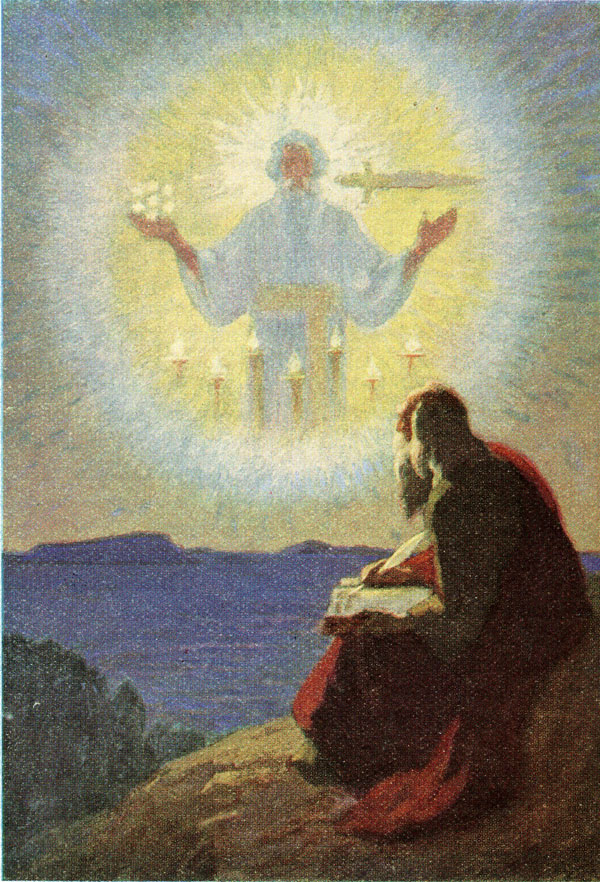
\includegraphics[width=0.98\textwidth]{images/illustrations/fugelmenschensohn.jpg}
\end{center}